\documentclass[10pt, aspectratio=169]{beamer}
\usefonttheme{professionalfonts}
%\usetheme{CambridgeUS}
%
% Choose how your presentation looks.
%
% For more themes, color themes and font themes, see:
% http://deic.uab.es/~iblanes/beamer_gallery/index_by_theme.html
%
\mode<presentation>
{
  \usetheme{default}      % or try Darmstadt, Madrid, Warsaw, ...
  \usecolortheme{beaver} % or try albatross, beaver, crane, ...
  \usefonttheme{default}  % or try serif, structurebold, ...
  \setbeamertemplate{navigation symbols}{}
  \setbeamertemplate{caption}[numbered]
} 

\usepackage[english]{babel}
\usepackage[utf8x]{inputenc}
\usepackage{tikz}
\usepackage{pgfplots}
\usepackage{array}  % for table column M
\usepackage{makecell} % to break line within a cell
\usepackage{verbatim}
\usepackage{graphicx}
\usepackage{epstopdf}
\usepackage{amsfonts}
\usepackage{xcolor}
\usepackage[makeroom]{cancel}
%\captionsetup{compatibility=false}
%\usepackage{dsfont}
\usepackage[absolute,overlay]{textpos}
\usetikzlibrary{calc, angles,quotes}
\usetikzlibrary{pgfplots.fillbetween, backgrounds}
\usetikzlibrary{positioning}
\usetikzlibrary{arrows}
\usetikzlibrary{pgfplots.groupplots}
\usetikzlibrary{arrows.meta}
\usetikzlibrary{plotmarks}

\usepgfplotslibrary{groupplots}
\pgfplotsset{compat=newest} 
%\pgfplotsset{plot coordinates/math parser=false}

\usepackage{hyperref}
\hypersetup{
    colorlinks=true,
    linkcolor=blue,
    filecolor=magenta,      
    urlcolor=cyan,
}

%% 
\def\EXTERNALIZE{1} % for externalizing figures
\input{header.tex}

%% 
\title[EE 264]{Properties of LTI Systems}
\author{Jose Krause Perin}
\institute{Stanford University}
\date{June 29, 2018}

\begin{document}

\begin{frame}
  \titlepage
\end{frame}


\begin{frame}{Last lecture}
\begin{itemize}
	%\item We use random processes to model signals that cannot be easily described by simple equations
	\item A random process is an indexed collection of random variables
	\item A random process is strict-sense stationary (SSS) if all its finite-order statistics are time invariant. That's hard to verify in practice.
	\item A random process is wide-sense stationary (WSS) if its mean is constant and if its autocorrelation function only depends on the time difference. 
	\item A random process is ergodic if its time averages are equal to its probability averages
	\item The Fourier transform of the autocorrelation function is called the power spectrum density (PSD). The PSD has units of W/Hz or dBm/Hz.
	\item When a random signal is filtered by an LTI system defined by $h[n]\leftrightarrow H(e^{j\omega})$, its autocorrelation function is filtered by an LTI system defined by $h[n]\ast h^*[-n]$, and its PSD is shaped by $|H(e^{j\omega})|^2$
	\item Random processes that have PSD constant over all frequencies are called white noise
	\item By the central limit theorem, the output of an LTI system to a random input is approximately Gaussian distributed
\end{itemize}
\end{frame}

%
\begin{frame}{Today's lecture}
\tableofcontents
\end{frame}

%
\section{Magnitude and Phase Response}
\begin{frame}{Magnitude and phase response}
Recall that complex exponentials are \textbf{eigenfunctions} of LTI systems
\begin{equation*}
\mathrm{LTI}\{e^{j\omega n}\} = H(e^{j\omega})e^{j\omega n}
\end{equation*}

$H(e^{j\omega})$ is the corresponding \textbf{eigenvalue} of $e^{j\omega n}$

$H(e^{j\omega})$ tell us by how much the LTI system \textbf{scales} and \textbf{delays} $e^{j\omega n}$

\begin{equation*}
H(e^{j\omega}) = \underbrace{|H(e^{j\omega})|}_{\text{Magnitude}}\exp(j\underbrace{\arg H(e^{j\omega})}_{\text{Phase}}) \tag{polar coordinates}
\end{equation*}

\pause
Calculating the output $Y(e^{j\omega}) = H(e^{j\omega})X(e^{j\omega})$
\begin{align*}
|Y(e^{j\omega})| &= |H(e^{j\omega})|\cdot|X(e^{j\omega})| \tag{magnitudes multiply} \\ 
\arg Y(e^{j\omega}) &= \arg H(e^{j\omega}) + \arg X(e^{j\omega}) \tag{phases add}
\end{align*} 
\end{frame}

%
\begin{frame}{Magnitude and phase response}	
	\begin{center}
		\begin{tikzpicture}
		\node (img1) {\resizebox{0.6\linewidth}{!}{\includegraphics{figs/first_order_sys_freqz.eps}}};
		\node at ($(img1.north east) -(3cm, 0.75cm)$) {$20\log_{10}(|H(e^{j\omega})|)$};
		\node at ($(img1.east)-(3.2cm, 0.5cm)$) {$\angle H(e^{j\omega}) = \arg(H(e^{j\omega}))$};
		\end{tikzpicture}
	\end{center}
\end{frame}

%
\begin{frame}{Phase unwrapping}
	Calculating the phase $\angle H(e^{j\omega})$ using $\arctan(\cdot)$ leads to discontinuities known as \textbf{phase wrapping}, since the image of $\arctan(\cdot)$ is $[-\pi, \pi]$.
	
	\textbf{Phase unwrapping} corrects jumps of $\pm2\pi$ in the phase response.
	
	\begin{center}
		\resizebox{0.93\textwidth}{!}{\input{figs/phase_unwrapping.tex}}
	\end{center}	
	
\end{frame}

%
\begin{frame}{Group delay}
	\begin{block}{Definition}
		\begin{equation*}
			\tau_g(\omega) = \mathrm{grd}~ H(e^{j\omega}) \equiv -\dfrac{d}{d\omega}\mathrm{arg} H(e^{j\omega}) \tag{group delay}
		\end{equation*}
		
		Group delay measures by how much $e^{j\omega}$ is delayed by the LTI system. 
		
		In continuous-time, $\tau_g(\omega)$ has units of seconds. In discrete-time, $\tau_g(\omega)$ has units of samples.
	\end{block}
	
	\begin{block}{Example}
		If a system has linear phase:
		\begin{equation*}
			\mathrm{arg} H(e^{j\omega}) = -\omega n_d \tag{\textbf{linear phase}}
		\end{equation*} 
		
		Then, the group delay is constant:
		\begin{equation*}
		\tau_g(\omega) = -\dfrac{d}{d\omega}(-\omega n_d) = n_d \tag{\textbf{constant group delay}}
		\end{equation*} 
		
		\textbf{Conclusion:} Linear-phase systems delay all frequencies equally.	
	\end{block}
\end{frame}


\begin{frame}{Effect of group delay}
	Consider the \underline{causal} LTI system defined by the following $z$-transform
	\begin{align*}
	&H(z) = \\ &\bigg(\frac{(1-0.98e^{j0.8\pi}z^{-1})(1-0.98e^{-j0.8\pi}z^{-1})}{(1-0.8e^{j0.4\pi}z^{-1})(1-0.8e^{-j0.4\pi}z^{-1})}\bigg)\prod_{k=1}^4\bigg(\frac{(c_k^* -z^{-1})(c_k -z^{-1})}{(1 -c_kz^{-1})(1 -c_k^*z^{-1})}\bigg)^2
	\end{align*}
	where $c_k = 0.95e^{j(0.15\pi + 0.02\pi k)}$
	
	It has the following pole-zero plot:
	
	\begin{center}
		\resizebox{0.32\linewidth}{!}{\input{figs/group_delay_example.tex}}
	\end{center}
\end{frame}

%
\begin{frame}{Effect of group delay}
	\begin{block}{Wrapped and unwrapped phase response}
		\begin{center}
			\resizebox{0.55\linewidth}{!}{\includegraphics{figs/group_delay_example_phase.png}}
		\end{center}		
	\end{block}
\end{frame}

\begin{frame}{Effect of group delay}
	\begin{block}{Group delay and magnitude response}
		\begin{center}
			\resizebox{0.55\linewidth}{!}{\includegraphics{figs/group_delay_example_delay_magnitude.png}}
		\end{center}		
	\end{block}
\end{frame}

\begin{frame}{Effect of group delay}
	\begin{block}{Consider the following input signal}
		Three sinusoidal pulses of frequencies $\omega_1 = 0.8\pi$, $\omega_2 = 0.2\pi$, and $\omega_3 = 0.4\pi$.
		
	\begin{center}
		\begin{tikzpicture}
		\node (img1) {\resizebox{0.55\linewidth}{!}{\includegraphics{figs/group_delay_example_input.png}}};
		\node[fill=blue2!20, minimum width=1cm, scale=0.3] (l1) at ($(img1.north west)+(1.5cm, -0cm)$) {\Huge $\omega_1 = 0.8\pi$};
		\node[fill=red2!20, scale=0.3, right=0.25cm of l1] (l2) {\Huge $\omega_2 = 0.2\pi$};
		\node[fill=green2!20, scale=0.3, right=0.25cm of l2] (l3) {\Huge $\omega_3 = 0.4\pi$};
		\node[fill=blue2!20, minimum width=1cm, scale=0.3] (l4) at ($(img1.south east)+(-1.05cm, 2.8cm)$) {\Huge $\omega_1$};
		\node[fill=red2!20, minimum width=1cm, scale=0.3, left=1.6cm of l4] (l5)  {\Huge $\omega_2$};
		\node[fill=green2!20, minimum width=1cm, scale=0.3, left=1cm of l4] (l6)  {\Huge $\omega_3$};
		\end{tikzpicture}
	\end{center}	
	\end{block}
\end{frame}

\begin{frame}{Effect of group delay}
	\begin{center}
		\begin{tikzpicture}
		\node (img1) {\resizebox{0.42\linewidth}{!}{\includegraphics{figs/group_delay_example_delay_magnitude.png}}};
		\node[below=0cm of img1] (img2) {\resizebox{0.40\linewidth}{!}{\includegraphics{figs/group_delay_example_output.png}}};

		\node[fill=blue2!20, minimum width=1cm, scale=0.3] (l4) at ($(img1.north east)-(0.9cm, 0.5cm)$) {\Huge $\omega_1$};
		\node[fill=red2!20, minimum width=1cm, scale=0.3, left=1.2cm of l4] (l5)  {\Huge $\omega_2$};
		\node[fill=green2!20, minimum width=1cm, scale=0.3, left=0.7cm of l4] (l6)  {\Huge $\omega_3$};
		
		\node[fill=blue2!20, minimum width=1cm, scale=0.3] (l1) at ($(img1.south east)+(-0.9cm, 2.5cm)$) {\Huge $\omega_1$};
		\node[fill=red2!20, minimum width=1cm, scale=0.3, left=1.2cm of l1] (l2)  {\Huge $\omega_2$};
		\node[fill=green2!20, minimum width=1cm, scale=0.3, left=0.7cm of l1] (l3)  {\Huge $\omega_3$};
		
		\node[fill=blue2!20, minimum width=1cm, scale=0.3] (l7) at ($(img2.north east)+(-4.5cm, -0.25cm)$) {\Huge $\xcancel{\omega_1 = 0.8\pi}$};
		\node[fill=red2!20, scale=0.3, right=2.2cm of l7] (l9) {\Huge $\omega_2 = 0.2\pi$};
		\node[fill=green2!20, scale=0.3, right=0.7cm of l7] (l8) {\Huge $\omega_3 = 0.4\pi$};
	 
		\end{tikzpicture}
	\end{center}	
\end{frame}

\begin{frame}<beamer:0|handout:1>

Comments:
\begin{itemize}
	\item The sinusoidal pulse of frequency $\omega_1 = 0.8\pi$ was virtually eliminated, since $H(z)$ has a zero at frequency $0.8\pi$.
	\item The sinusoidal pulse of frequency $\omega_2 = 0.2\pi$ had a gain of about 1.2, but note that the group delay at that frequency is 150 samples.
	\item The sinusoidal pulse of frequency $\omega_3 = 0.4\pi$ had its amplitude doubled, but remained centered around $n = 150$, since the group delay of $H(z)$ around $0.4\pi$ is negligible.
	\item Interestingly, the effect of the system was to switch the position of the two pulses in time. Note that now, the pulse of frequency $\omega_3 = 0.4\pi$ comes before the pulse of frequency $\omega_2 = 0.2\pi$.
\end{itemize}

\end{frame}


%
\section{Poles, Zeros, and the Frequency Response}
\begin{frame}<beamer:1|handout:0>{Outline}
\tableofcontents[currentsection]
\end{frame}

\begin{frame}{Poles and zeros}

The \textbf{zeros} of $H(z)$ are the values of $z$ for which $H(z) = 0$, while the \textbf{poles} of $H(z)$ are the values of $z$ for which $H(z) = \infty$. 

For \textbf{rational $z$-transforms} (ratio of two polynomials in $z^{-1}$ or $z$), zeros and poles are the roots of the numerator and denominator polynomials, respectively.
\begin{align*}
H(z) &= \frac{B(z)}{A(z)} = \frac{b_0 + b_1z^{-1}+\ldots+b_Mz^{-M}}{a_0 + a_1z^{-1}+\ldots+a_Nz^{-N}} \\
&= \frac{b_0}{a_0}z^{N-M}\frac{(z-z_1)(z-z_2)\ldots(z-z_M)}{(z-p_1)(z-p_2)\ldots(z-p_N)}
\end{align*}
\begin{itemize}
	\pause\item If the coefficients $\{b_0, \ldots, b_M\}, \{a_0, \ldots, a_N\}$ are \underline{real}, the poles and zeros are either \underline{real} or they appear in \underline{complex conjugate pairs}
	\pause\item $H(z)$ has \textbf{finite impulse response (FIR)} if $a_k = 0, k = 1, \ldots N$ i.e., all poles of $H(z)$ are at the origin.
	\pause\item $H(z)$ has \textbf{infinite impulse response (IIR)} if $H(z)$ has poles away from the origin.
\end{itemize}	
\end{frame}

%
\begin{frame}{Poles, zeros, and the frequency response}

\textbf{Question:} How do poles and zeros affect the frequency response?

\textbf{Effect of a zero:} $H(z) = 1 - re^{j\theta}z^{-1}$

\begin{columns}[t]
	\begin{column}{0.55\textwidth}
		\vspace{-0.5cm}
		\begin{center}
			\resizebox{\linewidth}{!}{\input{figs/pole_zero_freq_resp.tex}}
		\end{center}
	\end{column}

	\begin{column}{0.3\textwidth}	
		\only<3|handout:1>{
		\textbf{Magnitude}
		\flushleft
		\begin{align*}
		H(z) &= \frac{z - re^{j\theta}}{z} \\
		|H(e^{j\omega})| &= \bigg|\frac{e^{j\omega} - re^{j\theta}}{e^{j\omega}}\bigg| \\
		&= \bigg|\bigg|\frac{{\color{red2} v_1} - {\color{black} v_2}}{{\color{red2} v_1}}\bigg|\bigg|\\
		&= \frac{||{\color{blue2} v_3}||}{||{\color{red2} v_1}||} \\
		&= ||{\color{blue2} v_3}||
		\end{align*}
	}

	\only<4|handout:2>{
	\textbf{Phase}
	\flushleft
	\begin{align*}
	H(z) &= \frac{z - e^{j\theta}}{z} \\
	\angle H(e^{j\omega}) &= \angle \frac{e^{j\omega} - re^{j\theta}}{e^{j\omega}} \\
	&= \angle(e^{j\omega} - re^{j\theta}) \\
	&- \angle e^{j\omega} \\
	&= \angle ({\color{red2} v_1}  - {\color{black} v_2}) - \angle {\color{red2} v_1} \\
	&= \angle {\color{blue2} v_3} - \omega
	\end{align*}
	}
	\end{column}
\end{columns}
\end{frame}

%
\begin{frame}{Poles, zeros, and the frequency response}
	
	\textbf{Effect of a pole:} $H(z) = \displaystyle\frac{1}{1 - re^{j\theta}z^{-1}}$
		
		\begin{columns}[t]
			\begin{column}{0.55\textwidth}
				\vspace{-0.5cm}
				\begin{center}
					\resizebox{\linewidth}{!}{\input{figs/pole_zero_freq_resp_pole.tex}}
				\end{center}
			\end{column}
			
			\begin{column}{0.3\textwidth}	
				\only<3|handout:1>{
					\textbf{Magnitude}
					\flushleft
					\begin{align*}
					H(z) &= \frac{z}{z - re^{j\theta}} \\
					|H(e^{j\omega})| &= \bigg|\frac{e^{j\omega}}{e^{j\omega} - re^{j\theta}}\bigg| \\
					&= \bigg|\frac{{\color{red2} v_1}}{{\color{red2} v_1} - {\color{black} v_2}}\bigg|\\
					&= \frac{||{\color{red2} v_1}||}{||{\color{blue2} v_3}||} \\
					&= \frac{1}{||{\color{blue2} v_3}||}
					\end{align*}
				}
				
				\only<4|handout:2>{
					\textbf{Phase}
					\flushleft
					\begin{align*}
					H(z) &= \frac{z}{z - re^{j\theta}} \\
					\angle H(e^{j\omega}) &= \angle \frac{e^{j\omega}}{e^{j\omega} - re^{j\theta}} \\
					&= -\angle(e^{j\omega} - re^{j\theta}) \\
					&+ \angle e^{j\omega} \\
					&= -\angle {\color{blue2} v_3} + \angle {\color{red2} v_1} \\
					&= -\angle {\color{blue2} v_3} + \omega
					\end{align*}
				}
			\end{column}
		\end{columns}
\end{frame}

%
\begin{frame}{Poles, zeros, and the frequency response}

Summary of effect of poles and zeros

\begin{center}
	\begin{tabular}{c|c|c}
	& Magnitude & Phase \\
	\hline
	Zero & $||{\color{blue2} v_3}||$ & $\angle {\color{blue2} v_3} - \omega$ \\
	Pole & $\displaystyle\frac{1}{||{\color{blue2} v_3}||}$ & $-\angle {\color{blue2} v_3} + \omega$ \\
	\hline
\end{tabular}
\end{center}

\begin{itemize}
	\pause\item As $e^{j\omega}$ approaches a zero, $|H(e^{j\omega})| \to 0$
	\pause\item As $e^{j\omega}$ approaches a zero, $\angle |H(e^{j\omega})|$ decreases ($- \omega$ factor).
	\pause\item At the zero there will be a negative-to-positive sign change of the phase response (\textbf{phase advance}) (must account effect of other zeros/poles)
	\pause\item As $e^{j\omega}$ approaches a pole, $|H(e^{j\omega})| \to \infty$
	\pause\item As $e^{j\omega}$ approaches a pole, $\angle |H(e^{j\omega})|$ increases ($+ \omega$ factor)
	\pause\item At the pole there will be a positive-to-negative sign change of the phase response (\textbf{phase lag}) (must account effect of other zeros/poles).	
\end{itemize}

\pause
\textbf{Conclusion:} Zeros decrease the magnitude and introduce phase advance (negative group delay), while poles increase magnitude and introduce phase lag (positive group delay)

\end{frame}

%
\begin{frame}{Poles, zeros, and the frequency response}
	Example: $H(z) = 1 - 0.9e^{j\pi/4}z^{-1}$
	\begin{center}
		\resizebox{0.93\linewidth}{!}{\input{figs/pole_zero_freq_resp_animation.tex}}
	\end{center}	
\end{frame}

\begin{frame}{Poles, zeros, and the frequency response}
	Example: $H(z) = 1 - 0.9e^{j\pi/4}z^{-1}$
	\begin{center}
		\resizebox{0.93\linewidth}{!}{\input{figs/pole_zero_freq_resp_animation_phase.tex}}
	\end{center}	
\end{frame}

\begin{frame}{Poles, zeros, and the frequency response}
	Example: $H(z) = \displaystyle\frac{1}{1 - 0.9e^{j\pi/4}z^{-1}}$
	\begin{center}
		\resizebox{0.93\linewidth}{!}{\input{figs/pole_zero_freq_resp_animation_pole.tex}}
	\end{center}	
\end{frame}

\begin{frame}{Poles, zeros, and the frequency response}
	Example: $H(z) = \displaystyle\frac{1}{1 - 0.9e^{j\pi/4}z^{-1}}$
	\begin{center}
		\resizebox{0.93\linewidth}{!}{\input{figs/pole_zero_freq_resp_animation_pole_phase.tex}}
	\end{center}	
\end{frame}

%
\begin{frame}{Match the pole-zero plots to the magnitude responses}
	\hspace*{-1cm}\resizebox{\paperwidth}{!}{\input{figs/match_pole_zero_mag_resp.tex}}
\end{frame}

%
\begin{frame}{Match the pole-zero plots to the phase responses}
	\hspace*{-1cm}\resizebox{\paperwidth}{!}{\input{figs/match_pole_zero_phase_resp.tex}}
\end{frame}

%
\begin{frame}{Sketch the magnitude and phase responses}
	\centering
	\resizebox{0.75\paperwidth}{!}{\input{figs/sketch_pole_zero_freq_resp.tex}}
\end{frame}

\begin{frame}{Important classes of LTI systems}

\begin{itemize}
	\item All-pass systems
	\item Minimum-phase systems
	\item Linear-phase systems
	\item Generalize linear-phase systems
\end{itemize}

\end{frame}

\section{All-Pass Systems}
\begin{frame}{All-pass systems}

\begin{block}{Definition}
	An all-pass system has magnitude response independent of $\omega$:
	\begin{equation*}
	|H(e^{j\omega})| = A = \text{Constant}, \forall \omega
	\end{equation*}
\end{block}

This condition is satisfied by systems of the form

\begin{align*}
H_{ap}(z) = \frac{z^{-1} - e_k^*}{1 - e_kz^{-1}} &= e_k^*\frac{z - 1/e_k^*}{z - e_k} \\
\text{pole at $e_k$} &\Longleftrightarrow \text{zero at $1/e_k^*$} 
\end{align*}

For every pole inside the unit circle $e_k$, there's a zero outside the unit circle at the \textbf{conjugate reciprocal} $1/e_k^*$ location. More generally,
\vspace{-0.25cm}
\begin{align*}
H_{ap}(z) = A\prod_{k = 1}^{M_r}\frac{z^{-1} - \tikz[baseline]{\node[fill=blue!10,anchor=base] {$d_k$};}}{1 - \tikz[baseline]{\node[fill=blue!10,anchor=base] {$d_k$};}z^{-1}}\prod_{k = 1}^{M_c}\frac{(z^{-1} - \tikz[baseline]{\node[fill=blue!20,anchor=base] {$e^*_k$};})(z^{-1} - \tikz[baseline]{\node[fill=blue!30,anchor=base] {$e_k$};})}{(1 - \tikz[baseline]{\node[fill=blue!20,anchor=base] {$e_k$};}z^{-1})(1 - \tikz[baseline]{\node[fill=blue!30,anchor=base] {$e^*_k$};}z^{-1})}
\end{align*}
$d_k$ are real poles and $e_k, e^*_k$ are complex conjugate poles.
\end{frame}

\begin{frame}{Causal all-pass systems properties}
\begin{enumerate}
	\item The unwrapped phase is always \underline{non-positive} (it may be zero)
	\begin{equation*}
	\arg(H_{ap}(e^{j\omega})) \leq 0, \qquad 0 \leq \omega\leq\pi
	\end{equation*}
	\item As a consequence of the above property, the group delay is always \underline{non-negative}
	
	\begin{equation*}
	\tau_g = -\dfrac{d}{d\omega}\arg(H_{ap}(e^{j\omega})) \geq 0, \qquad 0 \leq \omega\leq\pi
	\end{equation*} 
	
\end{enumerate}
\end{frame}

%
\begin{frame}{All-pass systems: example}
\begin{equation*}
H_{ap}(z) = \tikz[baseline]{\node[fill=blue!20,anchor=base] {$\displaystyle\frac{z^{-1}+ 0.75}{1 + 0.75z^{-1}}$};}\tikz[baseline]{\node[fill=red!20,anchor=base] {$\displaystyle\frac{z^{-1} - 0.5}{1 -0.5z^{-1}}$};}\tikz[baseline]{\node[fill=green!20,anchor=base] {$\displaystyle\frac{(z^{-1} - 0.8e^{-j\pi/4})(z^{-1} - 0.8e^{j\pi/4})}{(1 - 0.8e^{-j\pi/4}z^{-1})(1 - 0.8e^{j\pi/4}z^{-1})}$};}
\end{equation*}

\begin{center}
	\resizebox{\linewidth}{!}{\input{figs/allpass_zero_pole.tex}}
\end{center}
\end{frame}

\section{Minimum Phase Systems}
%
\begin{frame}{Minimum phase systems}
	\begin{block}{Definition}
		A \underline{causal} and \underline{stable} system is \textbf{minimum phase} if all its zeros are inside the unit circle.
	\end{block}

	As a consequence, if a system $H(z)$ is \textbf{minimum phase}, then the system $H^{-1}(z)$ (its inverse) is also causal, stable, and minimum phase.
	
\end{frame}

\begin{frame}{Properties of minimum phase systems}
\begin{enumerate}
	\item \textbf{Minimum phase-lag property} (the reason they are called minimum phase):
	
	\textit{Proof:}
	Any causal and stable $H(z)$ we can written as $H(z) = H_{min}(z)H_{ap}(z)$ (we'll see why in a few slides). The phase response is
	\begin{align*}
	\arg H(z) &= \arg H_{min}(z) + \arg H_{ap}(z) \tag{phases add} \\
	\arg H(z) &\leq \arg H_{min}(z) \tag{from properties of all-pass systems: $\arg H_{ap}(z) \leq 0$} \\
	-\arg H(z) &\geq -\arg H_{min}(z) \tag{phase lag $\equiv -\arg(\cdot)$}
	\end{align*} 
	\pause
	\textbf{Conclusion:} the systems $H(z)$ and $H_{min}(z)$ have the same magnitude response, but $H_{min}(z)$ has the minimum phase-lag response.
	\pause
	\item \textbf{Minimum group-delay property}: similarly to the property above. 
	\begin{align*}
	\mathrm{grd}~H(z) &= \mathrm{grd}~  H_{min}(z) + \mathrm{grd}~  H_{ap}(z) \tag{group delays add} \\
	\mathrm{grd}~  H(z) &\geq \mathrm{grd}~  H_{min}(z) \tag{from properties of all-pass systems: $\mathrm{grd}~  H_{ap}(z) \leq 0$}
	\end{align*} 
\end{enumerate}

\end{frame}


\begin{frame}{Properties of minimum phase systems}
\begin{enumerate}\setcounter{enumi}{2}
\item \textbf{Minimum energy-delay property}: The $N$ first samples of the impulse response of a minimum phase system $h_{min}[m] \leftrightarrow H_{min}(e^{j\omega})$ have more energy than the $N$ first samples of any other system $h[m]\leftrightarrow H(e^{j\omega})$ with same magnitude response. Formally,

If $|H_{min}(e^{j\omega})| = |H(e^{j\omega})|$, then
\begin{align*}
\sum_{m = 0}^{N-1} |h[m]|^2 \leq \sum_{m = 0}^{N-1} |h_{min}[m]|^2, \text{for any $N$}
\end{align*}

For proof, see problem 5.71 of the textbook.	
\end{enumerate}
\end{frame}


%
\begin{frame}{Minimum-phase/all-pass decomposition}
	Any rational system function $H(z)$ can be uniquely decomposed into a cascade of minimum phase system and an all-pass system:
	\begin{equation*}
	H(z) = H_{min}(z)H_{ap}(z)
	\end{equation*}
	
\textit{Proof sketch:}

Suppose that $H(z)$ has one zero outside the unit circle $1/c^*$. We can remove $1/c^*$ from $H(z)$ by simply writing
\begin{align*}
H(z) &= H_1(z)(z^{-1} - c^*) \\
&= \underbrace{H_1(z)(1 - cz^{-1})}_{\text{minimum phase}}\underbrace{\frac{z^{-1} - c^*}{1 - cz^{-1}}}_{\text{all-pass}}
\end{align*}

Since $|c| < 1$, the factor $H_1(z)(1 - cz^{-1})$ is also minimum phase and it differs from $H(z)$ only in that the zero of $H(z)$ that was outside the unit circle at $z = 1/c^*$ is reflected inside the unit circle to the conjugate reciprocal location $z = c$. 

This proof can be easily extended if $H(z)$ has more than one zero outside the unit circle.
	
\end{frame}

%
\begin{frame}{Algorithm for minimum-phase/all-pass decomposition}
Given a non-minimum phase system $H(z)$, we wish to find a minimum phase system $H_{min}(z)$ and an all-pass system $H_{ap}(z)$ such that
\begin{equation*}
H(z) = H_{min}(z)H_{ap}(z)
\end{equation*}
\begin{enumerate}
	\item Write $H_1(z)$, which contains all zeros and poles of $H(z)$ that are inside the unit circle.
	\item For each zero $1/c^*$ of $H(z)$ outside the unit circle, add a zero to $H_1(z)$ at the conjugate reciprocal location $c$. And add the term $\frac{z^{-1} - c^*}{1 - cz^{-1}}$ to the all-pass system.
	\item By convention, we make $|H_{ap}(z)| = 1$, so the gain of $H_{min}(z)$ at zero frequency must be equal to the gain of $H(z)$.
\end{enumerate}
\end{frame}

\begin{frame}{Example of minimum-phase/all-pass decomposition}
Consider the non-minimum phase system
\begin{equation*}
H(z) = \frac{(1 + \frac{3}{2}e^{j\pi/4}z^{-1})(1 + \frac{3}{2}e^{-j\pi/4}z^{-1})}{1 - \frac{1}{3}z^{-1}}
\end{equation*}
\begin{center}
	\resizebox{0.9\paperwidth}{!}{\input{figs/example_min_phase_allpass_decomp.tex}}
\end{center}
\end{frame}

\begin{frame}{Implications of minimum-phase/all-pass decomposition}
Suppose we want to design $H_d(z)$ to compensate for the effects of $H(z)$.

\begin{center}
	\resizebox{0.9\textwidth}{!}{
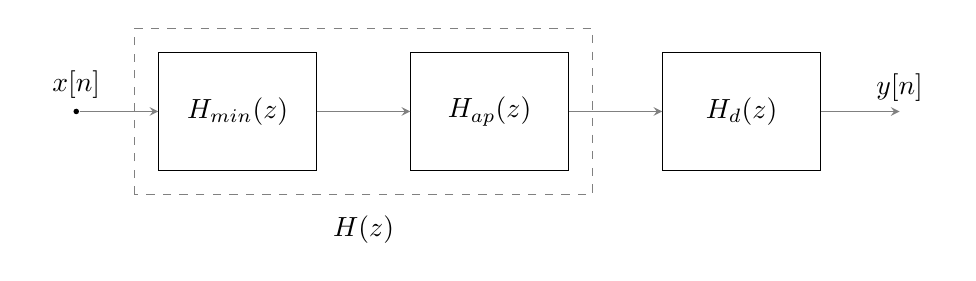
\begin{tikzpicture}[->, >=stealth, shorten >= 0pt, draw=black!50, node distance=3.2cm, font=\sffamily]
\tikzstyle{node}=[circle,fill=black,minimum size=2pt,inner sep=0pt]
\tikzstyle{block}=[draw=black,rectangle,fill=none,minimum size=1.5cm, inner sep=0pt]

\node[node] (xc) {};
\node[block, right=1cm of xc, text width = 2cm, align= center] (DSP1) {$H_{min}(z)$};
\node[block, right of= DSP1, text width = 2cm, align= center] (DSP2) {$H_{ap}(z)$};
\node[block, right of= DSP2, text width = 2cm, align= center] (DSP3) {$H_{d}(z)$};
\coordinate[right=1cm of DSP3] (yc) {};

\path (xc) edge (DSP1);
\path (DSP1) edge (DSP2);
\path (DSP2) edge (DSP3);
\path (DSP3) edge (yc);

\draw[dashed] ($(DSP1.south west) - (0.3cm,0.3cm)$) rectangle ($(DSP2.north east) + (0.3cm,0.3cm)$);
\node at ($(DSP1.west)!0.5!(DSP2.east)-(0, 1.5cm)$) {$H(z)$};

\node[above = 0mm of xc, text width = 1cm, align=center] {$x[n]$};
\node[above = 0mm of yc, text width = 1cm, align=center] {$y[n]$}; 
\end{tikzpicture}
}
\end{center}

Ideally, we'd like to have $H_d(z) = H^{-1}(z)$. But what if $H^{-1}(z)$ is \underline{unstable}?

\pause
\begin{equation*}
H_d(z) = H^{-1}_{min}(z)
\end{equation*}
Design $H_d(z)$ to compensate for the minimum phase system. $H^{-1}_{min}(z)$ is \underline{guaranteed to be stable}.

This choice of $H_d(z)$ compensates for the magnitude, but there'll still be an uncompensated phase distortion introduced by $H_{ap}(z)$. \textit{Oftentimes} that's good enough.
\end{frame}

\begin{frame}{Relation between magnitude and phase plots}

\textbf{Question:} given the magnitude response $|H(e^{j\omega})|$ of a \underline{causal} system, what can we tell about its phase response $\arg H(e^{j\omega})$?

\vspace{5mm}
\pause
For minimum phase systems, the magnitude response \underline{perfectly} describes the phase response.

\end{frame}

\begin{frame}{Kramers-Kronig relations}

For any \underline{real} and \underline{causal} system defined by $h(t) \leftrightarrow H(j\Omega) = H_r(j\Omega) + jH_i(j\Omega)$, where $H_r(j\Omega) = \mathrm{Re}\{H(j\Omega)\}$ and $H_i(j\Omega) = \mathrm{Im}\{H(j\Omega)\}$,

the \textbf{Kramers-Kronig relations} establish that
\begin{equation*}
H(j\Omega) = H_r(j\Omega) - j\mathcal{H}\{H_r(j\Omega)\},
\end{equation*}
where $\mathcal{H}\{\cdot\}$ is the \textbf{Hilbert transform}.

\pause
\textbf{Conclusion:} The imaginary part of $H(j\Omega)$ is determined from the Hilbert transform of the real part. Knowing just the real part is sufficient to completely specify the system, and the imaginary part is ``redundant'' information.

\pause
\begin{itemize}
	\item $H_r(j\Omega)$ is the Fourier transform of the even part of the impulse response, and  $H_i(j\Omega)$ is the Fourier transform of the odd part of the impulse response (recall even/odd decomposition from lecture 1)
	\item \textbf{Causality check}: compare the imaginary part of the frequency response with the Hilbert transform of the real part.
	\item All physical systems are causal, so the Kramers-Kronig relations apply to all physical LTI systems.
\end{itemize}
\end{frame}

\begin{frame}{The Hilbert transform}

The Hilbert transform of a signal $x(t)$ is defined as

\begin{equation*}
\mathcal{H}\{x(t)\} = h_{HT}(t)\ast x(t),
\end{equation*}

where 
\begin{equation*}
h_{HT}(t) = \begin{cases}
\frac{1}{\pi t}, & t \neq 0 \\
0, & t = 0
\end{cases}
\end{equation*}

\begin{equation*}
\mathcal{F}\{h_{HT}(t)\}  = H_{HT}(\Omega) = -j\mathrm{sign}(\Omega) = \begin{cases}
-j, & \Omega > 0 \\
0, & \Omega = 0 \\
j, & \Omega < 0
\end{cases}
\end{equation*}

More generally, the Hilbert transform is an operation over a function of some variable. If that function is $H(j\Omega)$ we would have

\begin{equation*}
\mathcal{H}\{H(j\Omega)\} = h_{HT}(\Omega)\ast H(j\Omega)
\end{equation*}

\end{frame}

\begin{frame}{Relating magnitude and phase responses}

\begin{align*}
H(e^{j\omega}) &= |H(e^{j\omega})|\exp(j\arg(H(e^{j\omega}))) \\
\ln H(e^{j\omega}) &= \underbrace{\ln |H(e^{j\omega})|}_{\text{real}} + j\underbrace{\arg(H(e^{j\omega}))}_{\text{imaginary}} \tag{taking $\ln$ of both sides}
\end{align*}

Now we could use the Kramers-Kronig relation to obtain
\begin{align*}
\arg(H(e^{j\omega})) &= -\mathcal{H}\{\ln |H(e^{j\omega})|\} \\
\end{align*}

The Kramers-Kronig relations only hold if $\ln H(e^{j\omega})$ is \underline{causal}. It turns out that if $H(e^{j\omega})$ is \underline{minimum phase}, then  $\ln H(e^{j\omega})$ is causal and we can apply the Kramers-Kronig relation.

\textbf{Conclusion:} The phase response of a minimum phase system is related to the  log-magnitude by the Hilbert transform.

%\textbf{Applications:} Phase retrieval problems. In many applications its is only feasible to measure intensity (magnitude). Examples: 

\end{frame}

\begin{frame}
Recall from the minimum phase/all-pass decomposition
\begin{align*}
H(e^{j\omega}) &= H_{min}(e^{j\omega})H_{ap}(e^{j\omega}) \\
|H(e^{j\omega})| &= |H_{min}(e^{j\omega})|\cancelto{1}{|H_{ap}(e^{j\omega})|} \\
\end{align*}

Therefore, if we apply the above procedure to a non-minimum phase system $H(z)$, we will recover the phase of its minimum phase component $H_{min}(z)$.
\end{frame}

%\begin{frame}{Example: plant identification by noise injection}
%
%\begin{center}
%	\resizebox{0.5\linewidth}{!}{\SimpleSys{figs/simple_in_dsp_out}{$x[n]$}{$H(z) = ??$}{$y[n]$}}
%\end{center}
%
%\textbf{Question:} how to estimate $H(z)$ without applying an impulse to the input?
%
%\pause
%Inject a small noise of known PSD $\Phi_{xx}(e^{j\omega})$ at the input and measure the noise PSD at the output $\Phi_{yy}(e^{j\omega})$:
%
%\begin{equation*}
%|H(e^{j\omega})|^2 = \frac{\Phi_{yy}(e^{j\omega})}{\Phi_{xx}(e^{j\omega})} \tag{only know the magnitude}
%\end{equation*}
%
%We can obtain the phase response by applying the method above:
%\begin{equation*}
%\arg(H(e^{j\omega})) = -\mathcal{H}\{\ln |H(e^{j\omega})|\}
%\end{equation*}
%
%This procedure only works if $H(z)$ is causal and minimum phase i.e., it is stable and has a stable inverse.
%
%\end{frame}

\section{Linear and Generalized Linear Phase Systems}
\begin{frame}<beamer:1|handout:0>{Outline}
\tableofcontents[currentsection]
\end{frame}

%
\begin{frame}{Linear-phase systems}
\begin{block}{Definition}
	\begin{equation*}
	H(e^{j\omega}) = |H(e^{j\omega})|e^{-j\omega\alpha}
	\end{equation*} 
\end{block}

The phase is a linear function of $\omega$: $\arg H(e^{j\omega}) = -\alpha\omega$. Consequently, the group delay is constant: $\mathrm{grd}~H(e^{j\omega}) = \alpha$.

\vspace{2mm}

This definition of linear-phase systems fails to include simple cases. \textbf{Example:} When  $H(e^{j\omega})$ is purely real, changes of sign in $H(e^{j\omega})$ cause jumps of $\pm\pi$ in $\mathrm{grd}~H(e^{j\omega})$. Hence, those systems are not strictly linear phase.

\end{frame}

\begin{frame}{Generalized linear phase systems}
\begin{block}{Definition}
	\begin{equation*}
	H(e^{j\omega}) = |H(e^{j\omega})|e^{-j\omega\alpha + j\beta}
	\end{equation*} 
	a term $\beta$ is added to account for constant phase changes. The phase function is now \textit{affine}.
\end{block}

\begin{align*}
\arg H(e^{j\omega}) &= \beta - \alpha\omega, 0 < \omega < \pi \tag{phase}\\
\mathrm{grd}~H(e^{j\omega}) &= \alpha \tag{group delay}
\end{align*}
\end{frame}

\begin{frame}{Ideal delay}

Consider the system with frequency response
\begin{equation*}
H(e^{j\omega}) = e^{-j\alpha\omega}, 0 \leq \omega \leq \pi \tag{ideal delay}
\end{equation*}

If $\alpha$ is \underline{integer}:
\begin{equation*}
h[n] = \delta[n-\alpha] \tag{from DTFT delay property}
\end{equation*}

If $\alpha$ is \underline{not integer}:
\begin{equation*}
h[n] = \frac{\sin \pi(n-\alpha)}{\pi(n-\alpha)} = \mathrm{sinc}(n-\alpha)
\end{equation*}

What does \underline{not integer} delay mean?

\end{frame}

%
\begin{frame}{Ideal delay}
\only<1|handout:1>{If $\alpha$ is \underline{integer}, delay corresponds to shifting samples.}
\onslide<2|handout:2>{If $\alpha$ is \underline{not integer}, delay corresponds to \textit{resampling}. Other samples are used to interpolate signal to obtain the value at the non-integer instants.}
\begin{center}
	\resizebox{0.6\linewidth}{!}{\input{figs/non-integer_delay.tex}}
\end{center}
\end{frame}

\begin{frame}{Interpretation of non-integer delay}

These two systems are equivalent. 

\begin{center}
	\resizebox{0.7\textwidth}{!}{
		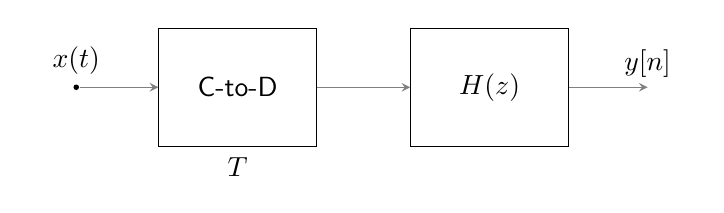
\begin{tikzpicture}[->, >=stealth, shorten >= 0pt, draw=black!50, node distance=3.2cm, font=\sffamily]
		\tikzstyle{node}=[circle,fill=black,minimum size=2pt,inner sep=0pt]
		\tikzstyle{block}=[draw=black,rectangle,fill=none,minimum size=1.5cm, inner sep=0pt]
		
		\node[node] (xc) {};
		\node[block, right=1cm of xc, text width = 2cm, align= center] (DSP2) {C-to-D};
		\node[block, right of= DSP2, text width = 2cm, align= center] (DSP3) {$H(z)$};
		\coordinate[right=1cm of DSP3] (yc) {};
		
		\path (xc) edge (DSP2);
		\path (DSP2) edge (DSP3);
		\path (DSP3) edge (yc);
		
		\node at ($(DSP2.south) - (0cm, 0.25cm)$) {$T$};
		\node[above = 0mm of xc, text width = 1cm, align=center] {$x(t)$};
		\node[above = 0mm of yc, text width = 1cm, align=center] {$y[n]$}; 
		\end{tikzpicture}
	}
\end{center}

\begin{center}
	\resizebox{\textwidth}{!}{
		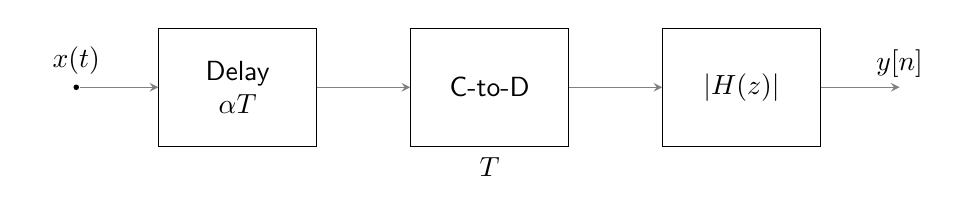
\begin{tikzpicture}[->, >=stealth, shorten >= 0pt, draw=black!50, node distance=3.2cm, font=\sffamily]
		\tikzstyle{node}=[circle,fill=black,minimum size=2pt,inner sep=0pt]
		\tikzstyle{block}=[draw=black,rectangle,fill=none,minimum size=1.5cm, inner sep=0pt]
		
		\node[node] (xc) {};
		\node[block, right=1cm of xc, text width = 2cm, align= center] (DSP1) {Delay \\ $\alpha T$};
		\node[block, right of= DSP1, text width = 2cm, align= center] (DSP2) {C-to-D};
		\node[block, right of= DSP2, text width = 2cm, align= center] (DSP3) {$|H(z)|$};
		\coordinate[right=1cm of DSP3] (yc) {};
		
		\path (xc) edge (DSP1);
		\path (DSP1) edge (DSP2);
		\path (DSP2) edge (DSP3);
		\path (DSP3) edge (yc);
		
		\node at ($(DSP2.south) - (0cm, 0.25cm)$) {$T$};
		\node[above = 0mm of xc, text width = 1cm, align=center] {$x(t)$};
		\node[above = 0mm of yc, text width = 1cm, align=center] {$y[n]$}; 
		\end{tikzpicture}
	}
\end{center}
\end{frame}

\begin{frame}{Causal FIR Linear-phase systems}

\textbf{Types I \& II: even symmetry}
\begin{align}
h[M-n] &= h[n], 0 \leq n \leq M \tag{even symmetry} \\
H(e^{j\omega}) &= A_e(e^{j\omega})e^{-j\omega M/2} \tag{Delay of $M/2$} \\
A_e(e^{j\omega}) &= A_e(e^{-j\omega}) \tag{due to even symmetry}
\end{align}

\begin{columns}
	\begin{column}{0.5\textwidth}
		Type I: $M$ even, integer delay
	\end{column}
	\begin{column}{0.5\textwidth}
		Type II: $M$ odd, half sample delay
	\end{column}
\end{columns}

\begin{center}
	\resizebox{\linewidth}{!}{\input{figs/fir_typeI-II.tex}}
\end{center}

\end{frame}

\begin{frame}{FIR Linear-phase systems}

\textbf{Types III \& IV: odd symmetry}
\begin{align}
h[M-n] &= -h[n], 0 \leq n \leq M \tag{odd symmetry} \\
H(e^{j\omega}) &= jA_o(e^{j\omega})e^{-j\omega M/2} \tag{Delay of $M/2$} \\
A_o(e^{j\omega}) &= -A_o(e^{-j\omega}) \tag{due to odd symmetry}
\end{align}

\begin{columns}
	\begin{column}{0.5\textwidth}
		Type III: $M$ even, integer delay
	\end{column}
	\begin{column}{0.5\textwidth}
		Type IV: $M$ odd, half sample delay
	\end{column}
\end{columns}

\begin{center}
	\resizebox{0.9\linewidth}{!}{\input{figs/fir_typeIII-IV.tex}}
\end{center}

\end{frame}

\begin{frame}{Summary of linear phase FIR systems}

\begin{center}
	\resizebox{\linewidth}{!}{
\begin{tabular}{c|c|c}
	& Even symmetry & Odd symmetry \\
	\hline
	$M$ even & Type I & Type III \\
	 & & zeros at $z = \pm 1$ \\
	 \hline
	$M$ odd & Type II & Type IV  \\
	& zeros at $z = -1$ & zeros at $z = +1$ \\
	\hline
	& $H(z^{-1}) = z^{M}H(z)$ & $H(z^{-1}) = -z^{M}H(z)$ 
\end{tabular}
}
\end{center}

\end{frame}

\begin{frame}{Question from midterm 2014}
\vspace{-0.5cm}
\begin{columns}
	\begin{column}{0.66\textwidth}
		\begin{figure}
			\includegraphics[height=0.85\textheight]{figs/midterm_14_poles_zeros.jpg}
		\end{figure}
	\end{column}
	\begin{column}{0.4\textwidth}
		\begin{enumerate}
			\item Which systems are FIR?
			\item Which ones are stable?
			\item Which ones are \textit{likely} all-pass?
			\item Which ones are minimum-phase?
			\item Which ones are \textit{likely} linear phase systems?
			\item Which ones could be Type II lowpass linear phase systems?
			\item Which ones likely have highpass frequency response?
		\end{enumerate}
	\end{column}
\end{columns}
\end{frame}

\begin{frame}{Summary}
\begin{itemize}
	\item The frequency response of a system tell us how much each frequency was scaled (magnitude response), and delayed (phase response) by the system.
	\item Poles increase magnitude and introduce phase lag (positive group delay)
	\item Zeros decrease the magnitude and introduce phase lead (negative group delay)
	\item All-pass systems have constant magnitude response. For each pole at $e_k$, there will be a zero at $1/e^*_k$ (conjugate reciprocal)
	\item Minimum phase systems have all zeros inside the unit circle. Hence, its inverse is stable.
	\item Any system can be decomposed into a cascade of a minimum phase system and an all-pass system
	\item For minimum phase systems, the phase response is given by the Hilbert transform of the log-magnitude response. 
	\item The phase response of a generalized linear phase systems is an affine function
	\item FIR systems are linear phase as long as their impulse response is symmetric
	\item Linear phase rational IIR systems do not exist
\end{itemize}
\end{frame}

\end{document}
